\section{Characterization method and results}
\label{Method}
% The setup of the experiment and preanalysis are discussed in sec.~\ref{sec:laserstage}. Analysis method and results of parameters are introduced in the following sections.
\subsection{Setup and preanalysis}
\label{sec:laserstage}

To obtain single PE events, the laser intensity is adjusted to the level of $\frac{1}{20}$ occupancy. The window size $T_{\mathrm{wave}}$ is \SI{10400}{ns} to include all the possible after-pulses (sec.~\ref{sec:afterpulse}). The rising edge of trigger waveform from the laser system is linearly interpolated to get the half-height time $t_{\mathrm{trig}}$ at about \SI{200}{ns} as shown in Fig.~\ref{fig:triggertime}.
\begin{figure}[!htbp]
    \centering
    \includegraphics[width=\LF\textwidth]{figures/method/triggerwave.pdf}
    \caption{An example of waveform and trigger signals. The orange line is the trigger waveform, with its high and low voltages indicated by two black horizontal dashed lines. The green cross is the interpolated trigger time. The blue solid line shows the PMT waveform with a PE pulse. The horizontal violet dotted line is the voltage threshold for calculating the baseline shown by the blue horizontal dashed line. Linearly interpolated 10\% and 90\% of (downward) rising and falling edges are represented by the green and cyan rectangles. Red and yellow vertical dashed lines respectively are the 10\% rising edge and the pulse peak.}
    \label{fig:triggertime}
\end{figure}


In the preanalysis, we select a preliminary window $[t_{\mathrm{trig}},600\,\mathrm{ns}]$ where dark noises (\SI{\sim 10}{kHz} in sec.~\ref{sec:dcr}) and laser pulses are expected to contribute 0.004 and 0.05 counts on average. The peak time $t_p$ is the position of minimum in each window as shown in Fig.~\ref{fig:triggertime}.
%Because the maximum pulse is selected in each waveform, the expected charge distribution is the distribution of $\max(C_n)$ ($n=1,...,N$), in which $C_n$ is the charge of the nth PE and $N$ is the number of PE in a waveform.



The baseline not being zero, we estimated it from the sidebands $[-200\,\mathrm{ns},-10\,\mathrm{ns}]$ and $[100\,\mathrm{ns},200\,\mathrm{ns}]$ relative to $t_p$. To remove potential additional pulses in the sidebands, from a rough estimation of white noise we define a voltage threshold shown as the horizontal voilet dotted line in Fig.~\ref{fig:triggertime} and cut off additional \SI{10}{ns} around each over-threshold time interval. The baseline $\mu_b$ is estimated as the average of the residual sidebands. The peak height $V_p$ of a pulse is the difference between $\mu_b$ and the minimum voltage.

To further reduce the dark noises, a gaussian $f(t;t_0,\sigma_{t0}^2)$ is fitted to the distribution of $t_p-t_{\mathrm{trig}}$ of pulses whose $V_p$ exceeds \SI{5}{ADC} over all the waveforms. We define the new candidate window, which is about \SI{30}{ns} long, as $[t_0-5\sigma_{t0}, t_0+5\sigma_{t0}]$ to calculate new $t_p$ and $V_p$ by repeating the above procedures. With such a candidate window we shall carry out all the analysis in the following sections except pre/after-pulses.

\subsection{charge spectrum}
\label{sec:noisepeak}

Considering the rise and fall time distributions, the charge $Q$ of a pulse is the summation of the baseline-subtracted voltages in a time window $[-10, 75]$\,ns relative to $t_p$ as illustrated in the pink region of Fig.~\ref{fig:triggertime}. The input impedance being \SI{50}{\Omega}~\cite{CAENV1751}, the charge in the unit of Coulomb is $Q/\SI{50}{\Omega}$.

Such $Q$ in Fig.~\ref{fig:triggercharge} represents the charge of a single PE with negligible multi-PE contributions due to the low occupancy. A long tail is evident in the single-PE charge distribution, which is also reported by JUNO collaboration~\cite{JUNOMassTesting}. Zhang~et~al.~\cite{JUNOLongtail} proposed a phenomenological parameterization without dedicated consideration of the multiplication process of the PEs. The physical model and solution of the long tail will be discussed in our future publications.

To describe the peak shape of the $Q$ distribution, a gaussian function $f(Q;Q_0,\sigma^2_{Q_0})$ is fitted to the interval $[0.65Q_0, 1.35Q_0]$ via the modified least-square (MLS) method~\cite{Cowan1998StatisticalDA} as the red line in Fig.~\ref{fig:triggercharge}. To remove the influence of the pedestal and describe the long tail~\cite{JUNOLongtail}, pulses with $V_p>\SI{3}{ADC}$ and $Q>0.25Q_0$ are selected to calculate mean $\overline{Q}$ and sample variance $s^2_{C}$ of $Q$. $\overline{Q}$ is larger than $Q_0$.
% The $V_p$ distribution with \SI{1}{ADC} bin width in Fig.~\ref{fig:triggerpeak} 
Fig.~\ref{fig:triggercharge} illustrates \SI{3}{ADC} and 0.25$Q_0$ threshold are complementary to exclude some noises with small $V_p$ but large $Q$.

\begin{figure}[!htbp]
    \centering
    \begin{subfigure}[b]{\SF\textwidth}
        \includegraphics[width=\textwidth]{figures/method/triggercharge.pdf}
        \caption{}%PM
        \label{fig:triggercharge}
    \end{subfigure}
    \begin{subfigure}[b]{\SF\textwidth}
        % \includegraphics[width=\textwidth]{figures/method/triggerpeak.pdf}
        % \caption{}%PM
        % \label{fig:triggerpeak}
        \includegraphics[width=\textwidth]{figures/result/gainres.pdf}
        \caption{}
        \label{fig:totalchargeCompare}
    \end{subfigure}
    \caption{(a) The long-tailed single-PE charge distribution of an MCP-PMT. The entries around zero are waveforms with no signal. The vertical blue dashed line is the pedestal cut. The orange histogram is the selected waveforms with peak-height cut ($V_p>\SI{3}{ADC}$). The pink and green areas are respectively the fit intervals for the peak and vally parameters.% (b) Peak-height distribution of an MCP-PMT before~(blue) and after~(orange) charge cut in (a). The vertical green dashed line is the peak-height cut.
    (b) The charge and resolution ratios showing the effect of long tail. Geen and red crosses represent the reference PMT and MCP-PMTs.
    }
\end{figure}

\subsection{Gain and single PE resolution}
\label{sec:noisegain}

The gain of the main peak and the entire sample are respectively ${Q_0}/{\SI{50}{\Omega}}/e$ and ${\overline{Q}}/{\SI{50}{\Omega}}/e$, $e$ being the charge of an electron. The relative \emph{peak} and \emph{sample resolutions} $\nu_0$ and $\nu$ are defined as ${\sigma_{Q_0}}/{Q_0}$ and ${\sqrt{s^2_{C}}}/{\overline{Q}}$.

The gain of main peak of 9 MCP-PMTs are in the scale of 1E7. $\nu_0$ and $\nu$ of 9 MCP-PMTs are $0.25\pm0.02$ and $0.69\pm0.03$. The 2d distribution of $\overline{Q}/{Q_0}$ and $\nu/{\nu_0}$ in Fig.~\ref{fig:totalchargeCompare} shows $\overline{Q}$ is about 1.8 times $Q_0$ for the MCP-PMTs. The long tail worsens the relative resolution from $\nu_0=0.25$ to $\nu=0.69$, compared to 0.37 of the reference PMT.

\begin{figure}[!htbp]
    \centering
    \includegraphics[width=\MF\textwidth]{figures/result/gainres.pdf}
    \caption{The charge and resolution ratios showing the effect of long tail. Geen and red crosses represent the reference PMT and MCP-PMTs.}
    \label{fig:totalchargeCompare}
\end{figure}

\subsection{Peak-to-valley ratio}
A parabolic function is fitted to the valley based on MLS in the interval $[-0.15Q_0, 0.25Q_0]$ relative to the least-counted bin of the histogram between the pedestal and the main peak as shown in Fig.~\ref{fig:triggercharge}. The \emph{valley count} $N_v$ is defined as the minimum of the parabola and \emph{peak count} $N_p$ is the maximum of the Gaussian described in sec.~\ref{sec:noisepeak}. The peak-to-valley ratio~(P/V) ${N_p}/{N_v}$ shows the ability to discriminate between electronic noises and a PE signal. The average P/V of MCP-PMTs is about 5.8, significantly higher than that (about 2.4) of the reference PMT.

\subsection{Single electron response}
As shown in Fig.~\ref{fig:triggertime}, $t^{10}_r$, $t^{50}_r$, $t^{90}_r$ ($t^{10}_f$, $t^{50}_f$, $t^{90}_f$) are the times of interpolated 10\%, 50\%, and 90\% $V_p$ in the rising (falling) edge. The rise time, fall time and full width at half maximum~(FWHM) are defined as $t_r = t^{90}_r - t^{10}_r$, $t_f = t^{10}_f - t^{90}_f$ and $\mathrm{FWHM} = t^{50}_f - t^{50}_r$. Averages and standard deviations of rise time, fall time and FWHM are $3.71\pm0.15$\,ns, $15.6\pm1.8$\,ns and $9.07\pm0.63$\,ns for 9 MCP-PMTs.

\begin{figure}
    \centering
        \includegraphics[width=\MF\textwidth]{figures/method/triggerSER.pdf}
        \caption{A fitting result of a pulse.}%PM
        \label{fig:triggerser}
    % \begin{subfigure}[b]{\SF\textwidth}
    %     \includegraphics[width=\textwidth]{figures/result/tausigma.pdf}
    %     \caption{}%PM
    %     \label{fig:sigmaCompare}
    % \end{subfigure}
    % \caption{(a)  (b) $\tau$ versus $\sigma$ of 9 MCP-PMTs.}
\end{figure}
To get a smooth single electron response (SER), $V_p>\SI{3}{ADC}$, the charge filter $[0.5Q_0, 1000\mathrm{ADC\cdot ns}]$ and the FWHM filter $[2\,\mathrm{ns}, 15\,\mathrm{ns}]$ are used to avoid the noise and very large pulses. An \emph{exGaussian} distribution $f^N(t;\mu_{\mathrm{ser}},\sigma_\mathrm{ser}^2)\otimes f^{\mathrm{Exp}}(t;1/\tau_\mathrm{ser})$~\cite{Luo:2022xrd} is used to fit the SER as shown in Fig.~\ref{fig:triggerser}, in which $\mu_{\mathrm{ser}}$ is the time offset of the pulse, $\sigma_{\mathrm{ser}}$ and $\tau_{\mathrm{ser}}$ model the shape feature of SER. The results of $\tau_{\mathrm{ser}}$ and $\sigma_{\mathrm{ser}}$ of 9 MCP-PMTs are $7.2\pm1.0$ and $1.62\pm0.06$.

\subsection{Transit time spread}
The PEs from the photocathode drift to the MCP as shown in Fig.~\ref{fig:mcpelectron}. The drifting electric field and the PE trajectory are simulated by a simplified model consisting of a cathode at \SI{0}{V}, a focusing electrode at \SI{480}{V} and an MCP at \SI{528}{V}. The drift times of the PEs from the top of the photocathode with \SI{0}{eV} and \SI{3}{eV} kinetic energies are about \SI{21}{ns} and \SI{18}{ns} respectively. A PE entering an MCP channel is multiplied to be an observable pulse, while that hitting the surface of the MCP gets scattered inelastically into several secondary electrons or elastically into one single electron~\cite{Furman}. The scattered electrons drift in the electric field until entering the MCP channels finally to give delayed pulses~\cite{KM3NetTesting}. Multiple secondary electrons with different kinetic energies may cause two or more pulses due to different drift times of secondary electrons as shown in Fig.~\ref{fig:triggerTT2pulse}.

\begin{figure}[!htbp]
    \centering
    \begin{subfigure}[t]{\SF\textwidth}
        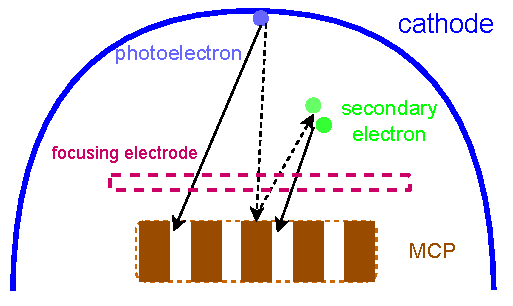
\includegraphics[width=\textwidth]{figures/method/MCPelectron.pdf}
        \caption{}%PM
        \label{fig:mcpelectron}
    \end{subfigure}
    \begin{subfigure}[t]{\SF\textwidth}
        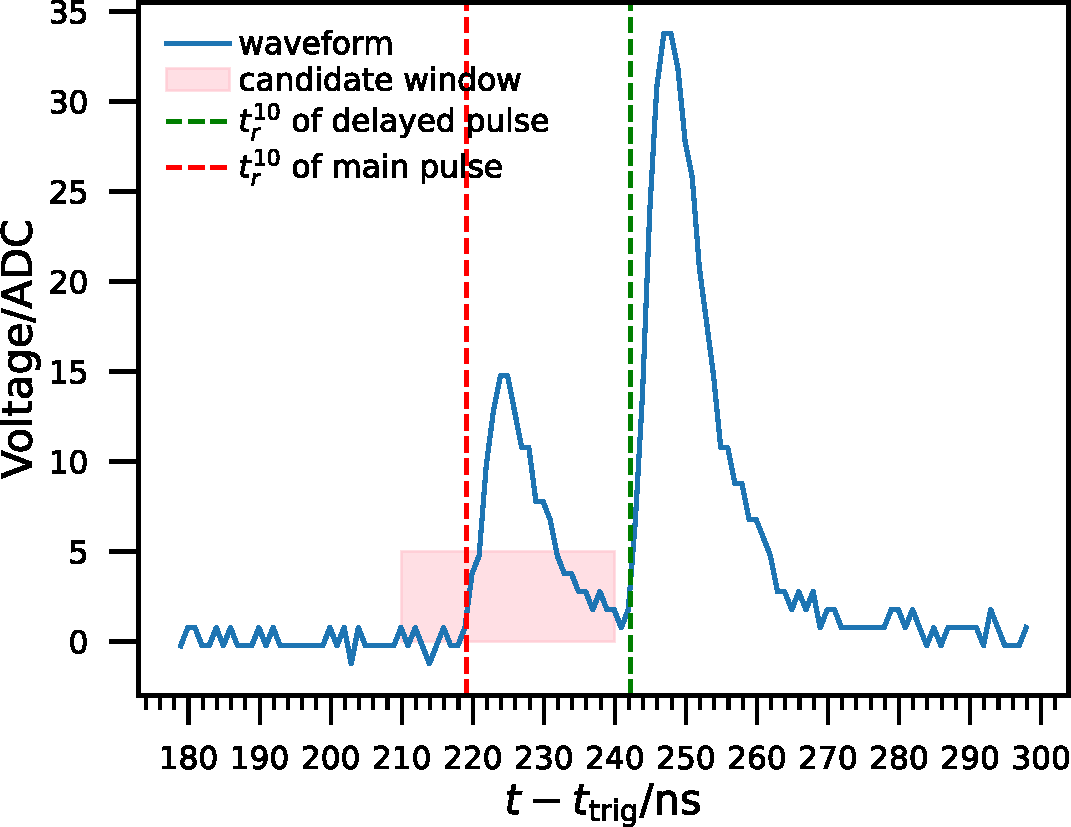
\includegraphics[width=\textwidth]{figures/method/triggerDoublePulse.pdf}
        \caption{}%PM
        \label{fig:triggerTT2pulse}
    \end{subfigure}
    \caption{(a) The PEs drift from the photocathode to the MCP and get amplified or scattered. (b) Double-pulse example. The first pulse falls in the candidate window defined in sec.~\ref{sec:laserstage}.}
\end{figure}

The transit time (TT) of a PE is the time needed to travel from the photocathode to the anode, mainly composed of the drift and multiplication times. However, the absolute TT is hard to measure. Practically, a relative $\mathrm{TT}$ is defined as the time difference between the trigger signal $t_{\mathrm{trig}}$ and 10\% rise time of a PE pulse $t_r^{10}$. The $\mathrm{TT}$ distribution of the MCP-PMTs contains slowly rising and falling edges on both sides of the peak as shown in Fig.~\ref{fig:triggerTTSLog} and \ref{fig:triggerTTS}. The rising edge is due to the PEs with larger kinetic energies while the falling one consists of secondary electrons with longer drift times~\cite{longtail}.

Delayed pulses are searched in the interval $[t_0+20\,\mathrm{ns},t_0+80\,\mathrm{ns}]$ to seperate them from the main pulses in $[t_0-5\,\mathrm{ns},t_0+5\,\mathrm{ns}]$. The blue histogram in Fig.~\ref{fig:triggerTTlatepulse} is the distribution of the delayed pulses and the filled one is for those with the main pulses in the same waveform. The sharp difference between them at about \SI{40}{ns} after the main peak, twice the drift time of PEs from the cathode to the MCP, reasonably illustrates that an elastically scattered electron cannot appear with a main pulse in the same waveform.

\begin{figure}[!htbp]
    \centering
    \begin{subfigure}[t]{\SF\textwidth}
        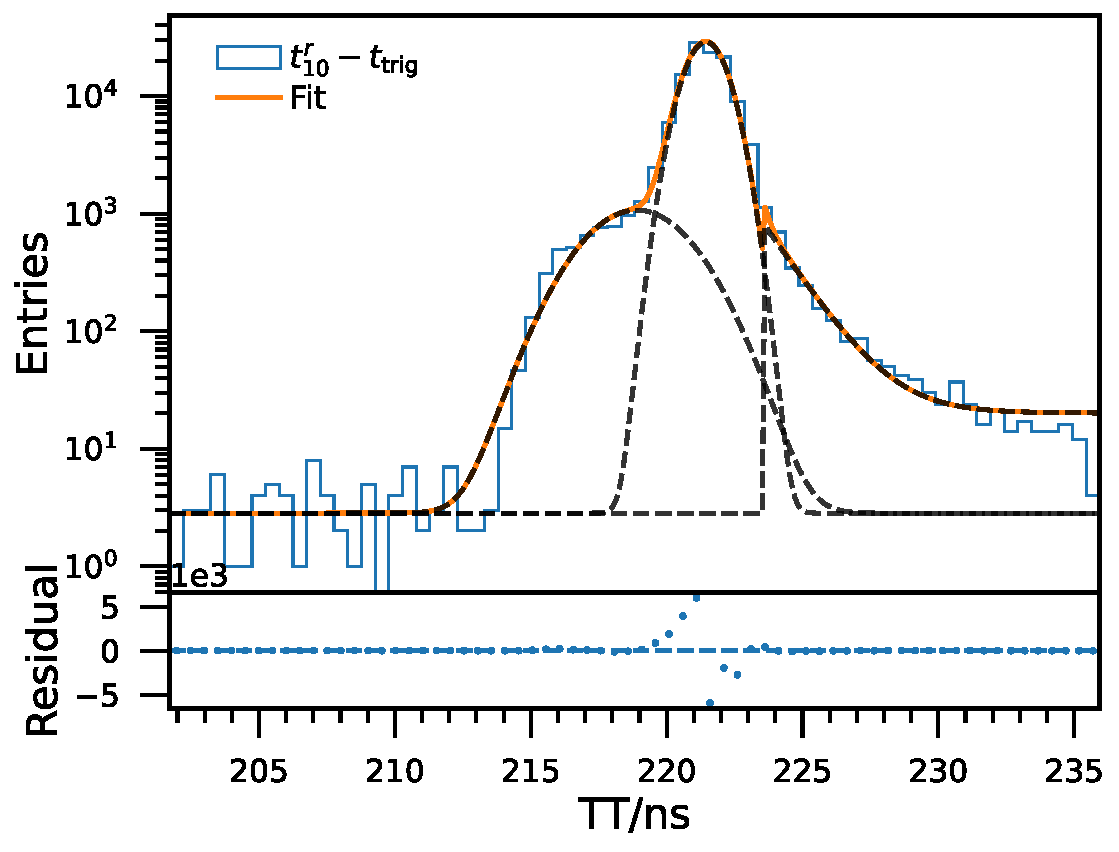
\includegraphics[width=\textwidth]{figures/method/triggerTTSLog.pdf}
        \caption{}%PM
        \label{fig:triggerTTSLog}
    \end{subfigure}
    \begin{subfigure}[t]{\SF\textwidth}
        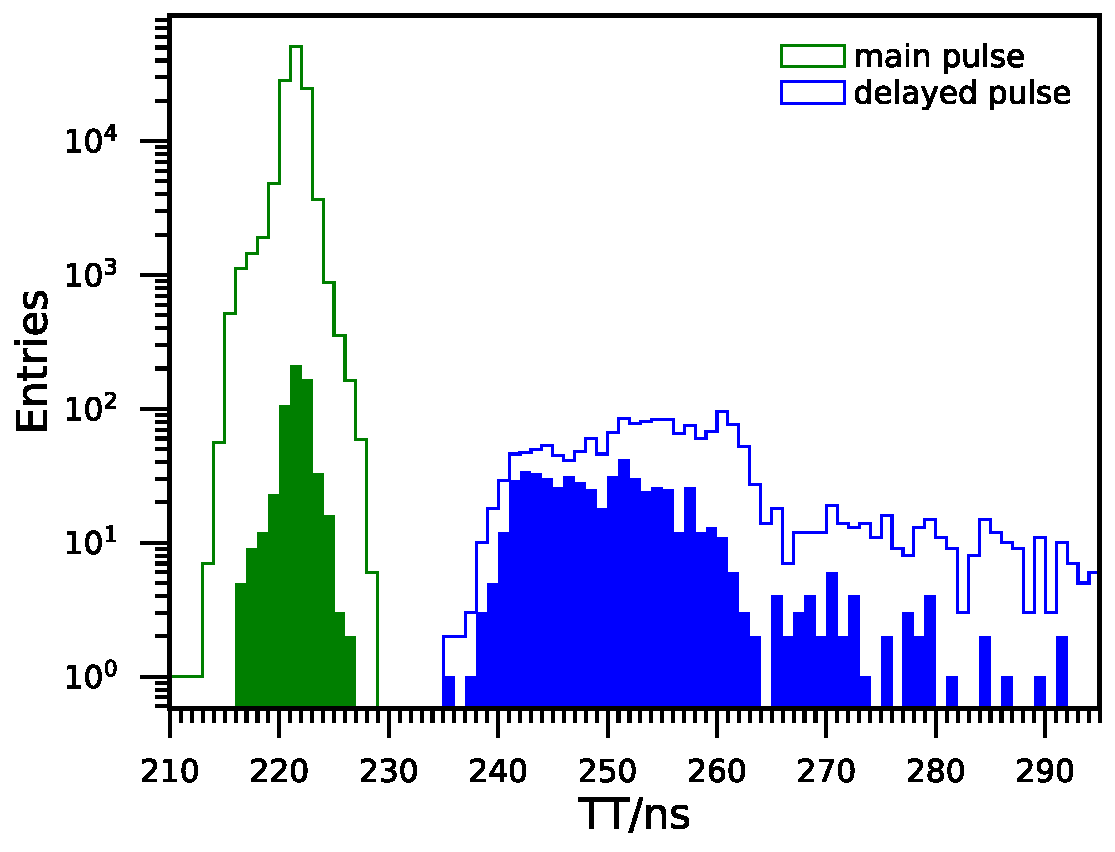
\includegraphics[width=\textwidth]{figures/method/triggerDelayedPulse.pdf}
        \caption{}%PM
        \label{fig:triggerTTlatepulse}
    \end{subfigure}
    \caption{(a) The distribution of TT with y-axis in logarithmic scale. The black dashed lines from left to right are early, main and delayed components with a dark noise pedestal. (b) The green and blue histograms are respectively the main and delayed pulse distributions. The filled histograms are waveforms containing the main and delayed pulses simultaneously.}
\end{figure}

The main and early components are modeled with Gaussians $N_1f_1^N(t;\mu_{\mathrm{TT}},\sigma_{\mathrm{TT}}^2)$ and $N_2f_2^N(t;\mu_K,\sigma_K^2)$, the subscript $K$ standing for PEs with high kinetic energies. Considering the exponential distribution of kinetic energies of secondary electrons~\cite{Furman,SecondElectron}, $f^\mathrm{Exp}(t;\tau_S)$ is suitable to model the delayed component.  We artificially add a constant $b_S$ and a translation of $\mu_{TT} + 2\sigma_{TT}$ to fit the data. As shown in Fig.~\ref{fig:triggerTTSLog} and Fig.~\ref{fig:triggerTTS}, the \SI{0.5}{ns}-binned histogram of $\mathrm{TT}$ is fitted by

\begin{equation}
    B+N_1f_1^N(t;\mu_{\mathrm{TT}},\sigma_{\mathrm{TT}}^2)+N_2f_2^N(t;\mu_K,\sigma_K^2)+b_SH(\mu_{\mathrm{TT}}+2\sigma_{\mathrm{TT}})+N_Sf^{\mathrm{Exp}}(t-(\mu_{\mathrm{TT}}+2\sigma_{\mathrm{TT}});1/\tau_S)
\end{equation}
in which $H$ is the heaviside function to limit definition domain of the delay component, $B$ is the constant dark noise rate. TTS is defined as FWHM $2\sqrt{2\ln(2)}\sigma_{\mathrm{TT}}$~\cite{HAMAMATSUManual} representing the timing resolution. The charge and TT seems to have some correlation in Fig.~\ref{fig:triggerTTS2d}, the long tail in charge distribution being evident in charge distribution.

\begin{figure}[!htbp]
    \centering
    \begin{subfigure}[t]{\SF\textwidth}
        \includegraphics[width=\textwidth]{figures/method/triggerTTS.pdf}
        \caption{}%PM
        \label{fig:triggerTTS}
    \end{subfigure}
    \begin{subfigure}[t]{\SF\textwidth}
        \includegraphics[width=\textwidth]{figures/method/triggerTTS2d.pdf}
        \caption{}%PM
        \label{fig:triggerTTS2d}
    \end{subfigure}
    \caption{(a) The distribution of TT with y-axis in linear scale. (b) The 2d distribution of TT and charge. The colorbar is in logarithmic scale.}
\end{figure}

\subsection{Dark count rate}
\label{sec:dcr}
The dark noise mainly comes from the spontaneous thermionic electrons emitted from the photocathode~\cite{KM3NetTesting} and mimick PEs. The dark count rate (DCR) is ${N_{\mathrm{noise}}}/({N_{\mathrm{hit}}T_{\mathrm{DCR}}})$, in which $N_{\mathrm{noise}}$ is the noise count in the interval of $[\SI{-200}{ns},\SI{-150}{ns}]$ relative to main pulse with $T_{\mathrm{DCR}}=\SI{50}{ns}$ and $N_{\mathrm{hit}}$ is the number of waveforms with main pulses. The DCR of 9 MCP-PMTs is $4.5\pm1.3\,\si{kHz}$.


\subsection{Pre-pulse and after-pulse}
\label{sec:afterpulse}
Generated from photons hitting the MCP or the first dynode directly rather than the photocathode, \emph{pre-pulses} appear about tens of nanoseconds earlier with smaller amplitudes~\cite{JUNOMassTesting}.

Ions such as \ce{H^+}, \ce{He^+}, \ce{O^+} produced from gaseous impurities in the vacuum blub by the PEs drift back to the photocathode, generate new electrons and further \emph{after-pulses}~\cite{JUNOMassTesting,Coates_1973}. The delay times of after-pulses are proportional to the square root of the mass-to-charge ratios of the ions~\cite{XENON1TTesting,Coates_1973,afterpulseTime}. %Considering electric field and $\frac{M}{Z}$ of ions, the travel time is in the scale of \si{us}.

The ratios of pre-pulses $R_{\mathrm{pre}}$ and after-pulses $R_{\mathrm{after}}$ are calculated in time interval [\SI{-100}{ns},\SI{-10}{ns}] ($T_{\mathrm{pre}}=90$\,ns) and [\SI{200}{ns},\SI{9800}{ns}] ($T_{\mathrm{after}}=9600$\,ns) relative to the main pulses respectively as following equations

\begin{align}
    R_{\mathrm{pre}} = \frac{N_{\mathrm{pre}}}{N_\mathrm{hit}} - \mathrm{DCR}\cdot T_{\mathrm{pre}}\\
    R_{\mathrm{after}} = \frac{N_{\mathrm{after}}}{N_\mathrm{hit}} - \mathrm{DCR}\cdot T_{\mathrm{after}}
\end{align}
in which $N_{\mathrm{pre}}$ and $N_{\mathrm{after}}$ are the number of pre-pulses and after-pulses. The small rate of pre-pulses is dominated by DCR at our low-occupancy setup.

\begin{figure}
    \centering
    \includegraphics[width=\LF\textwidth]{figures/method/triggerAfterpulseSchema.pdf}
    \caption{An example waveform for searching pre-pulses and after-pulses. Green and red vertical dashed lines are respectively the trigger time and 10\% of rising edge of main pulse $t_r^{10}$. The gray and orange regions are respectively the intervals for searching after-pulses and pre-pulses.}
    \label{fig:afterpulseSchema}
\end{figure}



The pre-pulses and after-pulses are searched from \SI{10}{ns} before and \SI{200}{ns} after the main pulse. The 10\% rise time $t_r^{10}$ and charge $Q$ of the after-pulse and pre-pulse are calculated in the $[-\SI{10}{ns},\SI{75}{ns}]$ window relative to the peak position as shown by violet area in Fig.~\ref{fig:afterpulseSchema}.

\begin{figure}[!htbp]
    \centering
    \begin{subfigure}[t]{\LF\textwidth}
        \includegraphics[width=\textwidth]{figures/method/triggerAfterpulse1d.pdf}
        \caption{}%PM
        \label{fig:afterpulse1d}
    \end{subfigure}
    \begin{subfigure}[t]{\LF\textwidth}
        \includegraphics[width=\textwidth]{figures/method/triggerAfterpulse2d.pdf}
        \caption{}
        \label{fig:afterpulse2d}
    \end{subfigure}
    \caption{(a) An example of time distributions of pre-pulses (orange) and after-pulses (blue) for an MCP-PMT, the green line being the Gaussian fits. The blank area around the \SI{0}{ns} is the main pulses not shown in this figure. (b) Charge versus time distribution of pre-pulses and after-pulses. The horizontal bright band at about 100\,$\mathrm{ADC}\cdot \mathrm{ns}$ mainly contains the dark noise.}
\end{figure}
% waveform analysis

The distribution of delay time from $t_r^{10}$ of main to after-pulse in Fig.~\ref{fig:afterpulse1d} indicates 4 characteristic peaks at around \SI{300}{ns}, \SI{550}{ns}, \SI{1200}{ns} and \SI{1700}{ns}, ratio being about $1:\sqrt{3}:\sqrt{16}:\sqrt{32}$. These peaks may originate from \ce{H^+}, \ce{He^{+}}, \ce{O^+} or \ce{CH_4^+}, and \ce{O_2^+} or \ce{Ar^+}. XENON1T~\cite{XENON1TTesting} and XMASS~\cite{Abe_2020} gave similar assumptions for the first two peaks. Similar works by JUNO~\cite{Zhao:2022gks} and KM3NeT~\cite{KM3NetTesting} claimed the first peak to be \ce{H_2^{+}}.%Double Chooz proposed an unclear assumption for those peaks for R7081 PMT~\cite{Haser_2013}.

We use 4 gaussians $\sum_{i=1}^{4}{A_if_i^{\mathrm{AP}}(t;t_i,\sigma_i^2)}$ to model the four peaks after substracting DCR,
in which $A_i$, $t_i$, and $\sigma_i$ are the amplitudes, times, width of each after-pulse peak (Table.~\ref{tab:afterpulse}). The amplitudes of the 4 peaks vary greatly for different MCP-PMTs in Fig.~\ref{fig:afterpulsePeak}. There are still unexplained structures, such as exponential component between the first and second peaks.
\begin{table}
    \centering
    \caption{Parameters of after-pulse of 9 MCP-PMTs}
    \label{tab:afterpulse}
    \begin{tabular}{c|c|c|c|c}
        \hline
        &1st peak&2nd peak&3rd peak&4th peak\\
        $t_i$/ns&305$\pm$6&563$\pm$21&1196$\pm$39&1722$\pm$24\\
        $A_i/A_1$&1&0.73$\pm$0.26&1.23$\pm$0.47&2.2$\pm$1.1\\
        $\sigma_i$/ns&8.8$\pm$2.1&82$\pm$29&61$\pm$24&69$\pm$26\\
        \hline
    \end{tabular}
\end{table}

\begin{figure}[!htbp]
    \centering
    \begin{subfigure}[t]{\SF\textwidth}
        \includegraphics[width=\textwidth]{figures/result/afterpulse.pdf}
        \caption{}%PM
        \label{fig:afterpulsePeak}
    \end{subfigure}
    \begin{subfigure}[t]{\SF\textwidth}
        \caption{}
        \label{fig:prepulseCompare}
    \end{subfigure}
    \caption{(a) Time and relative amplitudes of after-pulse peaks of 9 MCP-PMTs.}
\end{figure}

% Fig.\ref{fig:afterpulse2d} indicates that the after pulse contains some very large signal in the specific peaks, which is different from the distribution of single PE.




\subsection{Relative photon detection efficiency}
\label{sec:PDE}
 %For example, JUNO fixed one reference PMT to calibrate the light intensity and other reference PMTs are circulated through all channels to calibrate the light allocation ratio~\cite{Wonsak_2021}.
A regression method is developed to combine the light-source calibration and PDE measurements simultaneously with 1 reference PMT. Note $I_n$ to be the light intensity of the $n$-th run, $\alpha_j$ to be the light allocation ratio of the $j$-th splitter channel (out of 4) assumed to be stable across runs, $\eta_k$ to be the PDE of the $k$-th PMT (out of 1 reference dynode and 9 MCP PMTs). The PE counts in each waveform obey Poisson distribution $\pi(I_n\alpha_j\eta_k)$.

For convenience, the reference PMT is set to be the 0-th. Note $\alpha_j^0\equiv\alpha_j/{\alpha_0}$, $\eta_k^0\equiv\eta_k/{\eta_0}$, $I_n^0\equiv I_n\alpha_0\eta_0$.  The trigger rate $R_{njk}$ of the $k$-th PMT at the $j$-th channel in the $n$-th run is

\begin{equation}
    \label{equ:linkfunction}
    R_{njk}=1-\exp\left(-I_n\alpha_j\eta_k\right)=1-\exp\left(-e^{\log{I_n^0}+\log{\alpha_j^0}+\log{\eta_k^0}}\right).
\end{equation}

The trigger number $N^{\mathrm{trig}}_{njk}$ of the $k$-th PMT in the $n$-th run with the $j$-th splitter obey Binomial distribution $B(N^{\mathrm{trig}}_{njk};R_{njk},N^t_{njk})$, in which $N^t_{njk}$ is total number of waveforms by the laser trigger. The likelihood is therefore

\begin{equation}
    \label{equ:likelihood}
    \mathcal{L}=\prod_{njk}{R_{njk}^{N^\mathrm{hit}_{njk}}(1-R_{njk})^{N^t_{njk}-N^{\mathrm{hit}}_{njk}}}.
\end{equation}

The relationship in Equ.~\eqref{equ:linkfunction} and \eqref{equ:likelihood} defines a \emph{Binomial regression} with \emph{complenmentary log-log} link function~\cite{glm}, with $\log{\eta_k^0}$, $\log{\alpha_j^0}$ and $\log{I_n^0}$ as parameters. The relative PDEs $\eta_k^0$ of MCP-PMTs are calculated from the regression results to be about $1.71$, significantly higher than the reference PMT.
